\documentclass[9pt]{extarticle}

\usepackage[utf8]{inputenc}              % Tipos de caracteres
\usepackage[portuguese]{babel}           % Português
\usepackage[a4paper,portrait]{geometry}  % Tipo de papel
\usepackage{color}                       % Para tratamento da cor
\usepackage{graphicx}                    % Para a imagem
\DeclareGraphicsExtensions{.jpg,.png}
\usepackage{amsmath}                     % Para as matematiquices
\usepackage{amssymb}
\usepackage{array}
\usepackage{gensymb}                     % Grau
\usepackage{multicol}
\setlength{\columnsep}{1cm}
\usepackage{geometry}					% Margens
%\usepackage{xfrac}
\usepackage{colortbl}

\usepackage{multirow}

\addtolength{\topmargin}{-20mm}
\addtolength{\textheight}{55mm}
\addtolength{\oddsidemargin}{-15mm}
\addtolength{\textwidth}{32mm}

\renewenvironment{abstract}
 {\small
  \begin{center}
  \bfseries \abstractname\vspace{-.5em}\vspace{0pt}
  \end{center}
  \list{}{
    \setlength{\leftmargin}{0cm}%
    \setlength{\rightmargin}{\leftmargin}%
  }%
  \item\relax}
 {\endlist}
 
\renewcommand{\abstractname}{Resumo}
\renewcommand{\bibname}{Referências}

\delimitershortfall-1sp
\newcommand\abs[1]{\left|#1\right|}
\newcommand{\PR}[1]{\ensuremath{\left[#1\right]}}
\newcommand{\PC}[1]{\ensuremath{\left(#1\right)}}
\newcommand{\chav}[1]{\ensuremath{\left\{#1\right\}}}

\newcolumntype{x}[1]{>{\centering\hspace{0pt}}p{#1}}

\begin{document}

\title {\bf \huge T1 - Conversor Termoelétrico}
\author
{{\small Grupo III - João Ferreira (78179) Henrique Rodrigues (78632) Rodrigo C. Carvalho (78646) Cristina Melício (78947)} \\
{\small MEFT - 2ºAno, 2º Semestre - Laboratório de Complementos de Eletromagnetismo e Termodinâmica}}
\date{{\small Sexta-Feira, 13 de Março de 2015}}
\maketitle

\begin{abstract}
\par Neste trabalho foi efectuada a análise de um conversor termoeléctrico e o estudo do efeito de Peltier numa célula de Peltier que lhe estava associada. Conseguiu-se para este sistema actuando enquanto máquina térmica determinar o valor da resistência de carga óptima, diversos rendimentos do processo com diversos graus de aproximações ideiais, isto é, tendo em conta as diversas fontes de perda de potência do sistema, tais como a potência por condução, bem como a determinação da resistência térmica do sistema. Verificou-se que a um aumento de tensão corresponde uma maior diferença de temperaturas e por conseguinte um maior rendimento. Por fim, considerando o conversor actuando enquanto bomba térmica, calculou-se a sua eficiência para diversos valores de intensidade de corrente, verificando que a menores valores de intensidade de corrente corresponde uma maior eficiência.
\end{abstract}

\begin{multicols}{2}

\section{Introdução}

\par O conversor termoelétrico é um dispositivo que permite criar uma diferença de potencial a partir de uma diferença de temperaturas, e vice-versa. 

\par Os fenómenos que estão na explicação desta experiência são o efeito de \textit{Seeback}, de \textit{Peltier} e de \textit{Thomson}. O efeito de \textit{Seeback}, consiste em impor uma diferença de temperaturas  $\Delta T$ entre as placas condutoras nas extremidades da célula de modo a obter uma diferença de potencial, $V$, estando estas relacionadas pelo coeficiente de \textit{Seeback}:

\begin{equation}
S_{A,B} = \frac{V}{\Delta T}
\end{equation}

\par onde A e B correspondem aos materiais das extremidades. Já o efeito de \textit{Peltier} consiste em impor uma diferença de potencial à célula de modo a produzir um gradiente de temperatura entre as placas, estando a densidade de fluxo de calor resultante da existência deste gradiente de temperaturas, $J_Q$, relacionada com a corrente por unidade de área, J, pelo coeficiente de \textit{Peltier}:

\begin{equation}
\Pi_{A,B} = \frac{J_{Q_{A}}-J_{Q_{B}}}{J}
\end{equation}

\par A relação que se estabelece entre estes dois efeitos é conhecida pela Segunda Relação de Kelvin e é dada por:

\begin{equation}
\Pi_{A,B} = T S_{A,B}
\end{equation}

\par Revela-se necessário considerar ainda o efeito de \textit{Thomson} se existir grandiente do coeficiente de Seeback, ou seja, se este não depender linearmente com a temperatura. Sendo assim, o coeficiente de \textit{Thomson} é dado por:

\begin{equation}
\tau = \frac{\dot{q}_{Thomson}}{\vec{J} \cdot \vec{\nabla} T}
\end{equation}

\par A relação dada pelos três efeitos, denominada Primeira Relação de Kelvin, corresponde a:

\begin{equation}
\frac{d \Pi_{A,B}}{dT} + \tau_A - \tau_B = S_{A,B}
\end{equation}

\par Nesta experiência o conversor termoelétrico tem por base uma célula de \textit{Peltier} em contacto com duas placas condutoras de metais diferentes.

\par Na primeira parte, o mecanismo cujo esquema está representado na figura 1 é usado como máquina térmica, pelo que o seu rendimento é dado por:

\begin{equation} \label{n1}
\eta_1=\frac{P_2}{P_1}}
\end{equation}

\par onde $P_2$ e $P_1$ são, respetivamente, a potência dissipada na resistência $R_2$ (ligada à célula) e a potência fornecida pela fonte quente $E_1$, dadas pelas seguintes expressões:
\begin{gather}
P_1 = V_1 I_1 \\
P_2 = \frac{{V_2^2}}{R_{2_{0}}}
\end{gather}

\hspace{-0.8cm}
\begin{center}
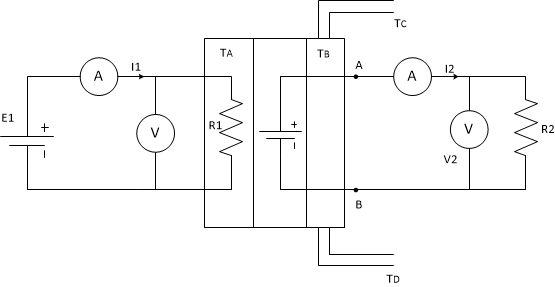
\includegraphics[width=220pt]{figura1.png}
\begin{center}
\par\noindent {\scriptsize ({\bf Figura 1}: Esquema da montagem da parte 1)}
\end{center}
\end{center}

Para maximizar o rendimento determina-se a resistência de carga ótima $R_{2{_0}}$, para a qual a potência $P_2$ é máxima, dada pela fórmula:

\begin{equation} \label{Ro}
R_{2{_0}} = \frac{5I_{2{_5}}-2I_{2{_2}}}{I_{2_2}-I_{2_5}} - 2 R_a
\end{equation}

onde $R_a$ é a resistência interna do amperímetro obtida pela fórmula:
\begin{equation}
R_a = \frac{V_a}{I_2} 
\end{equation}

\par Uma vez que existem perdas de energia, nem toda a potência fornecida pela fonte quente chega à fonte fria ou é transformada pela célula em corrente, sendo necessário considerar também a potência retirada da fonte fria pelo fluido de arrefecimento, ou seja, $ P_3$, que se obtém com seguinte equação:
\begin{equation} \label{P3}
P_3 = \dot{m} C (T_c-T_d)
\end{equation}

\begin{center}
\par\noindent {\scriptsize (Onde $C=4186Jkg^{-1}K^{-1}$ é a capacidade térmica mássica da água e $\dot{m}$ é o caudal do fluido de arrefecimento dado por
\begin{equation} \label{caudal}
\dot{m} = \frac{\rho V}{\Delta t}
\end{equation}
\par\noindent sendo $\rho$ a densidade da água)
}
\end{center}

\par Considerando uma potência dissipada dada por:
\begin{equation} \label{Pdiss}
P_{diss}=P_1-P_2-P_3
\end{equation}

\par\noindent tem-se a primeira correção ao rendimentos:
\begin{equation} \label{n2}
\eta_2=\frac{P_2}{P_1-P_{diss}}=\frac{P_2}{P_2+P_3}
\end{equation}

\par Para a última correção ao rendimento considera-se ainda que uma parte da potência passa da fonte quente para a fonte fria por condução através da célula fotovoltaica, obtendo a fórmula:
\begin{equation} \label{n3}
\eta_3=\frac{P_2}{P_2+P_3-P_{3_{cond}}}
\end{equation}
De forma a calcular a potência dissipada por condução considera-se uma resistência térmica entre a fonte fria $T_A$ e a quente $T_B$, cuja formula é:
\begin{equation} \label{Rt}
R_T = \frac{T_A - T_B}{P_{3_{cond}}}
\end{equation}
Para avaliar o desempenho da máquina tem-se como referência o rendimento do motor reversível operando entre as temperaturas das fontes.
\begin{equation} \label{Nc}
\eta_{Carnot} = 1 - \frac{T_B}{T_A}
\end{equation}

Na segunda parte da experiência, com base no efeito de \textit{Peltier}, o conversor, representado na figura 2, é utilizado como bomba de calor, sendo a eficiência, também denominada COP - \textit{coefficient of performance} -  determinada pela expressão:
\begin{equation} \label{e}
\varepsilon=\frac{P_3}{P_2}
\end{equation}
em que $P_2$ é a potência cedida pela fonte de tensão $E_2$ e é dada pela expressão:
\begin{equation}
P_2= V_2 I_2
\end{equation}

\hspace{-0.8cm}
\begin{center}
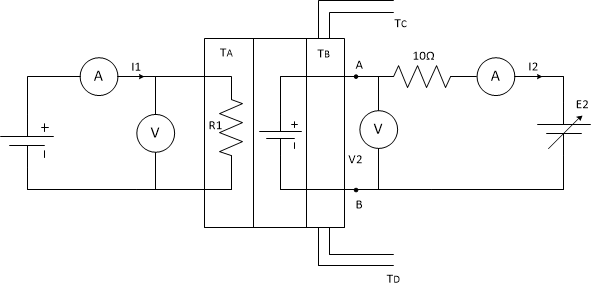
\includegraphics[width=220pt]{figura2.png}
\begin{center}
\par\noindent {\scriptsize ({\bf Figura 2}: Esquema da montagem da parte 2)}
\end{center}
\end{center}

A eficiência de referência é a da máquina de Carnot, cuja temperatura da fonte quente é $T_A$, e da fonte fria $T_B$, dada pela expressão:
\begin{equation} \label{ec}
\varepsilon_c = \frac{T_B}{T_B - T_A}
\end{equation}

\section{Dados Experimentais}

\subsection*{Conversor termoelétrico como máquina térmica}

\par Em primeiro lugar, pretendia-se determinar a resistência de carga ótima. Escolheu-se um valor de $5\Omega$ para a resistência $R_2$, e um valor de $10V$ para $E_1$. Observou-se a evolução da temperatura nos quatro canais, e aguardou-se até à sua estabilização.

\par Devido à susceptibilidade de variação de caudal, foi-se calculando o seu valor sempre que se retiravam outros valores, através da expressão \eqref{caudal}. Com um cronómetro mediu-se o tempo, e com uma proveta graduada mediu-se o volume de água.

\par Atingido o equilíbro, registou-se as quatro temperaturas, as tensões $V_1$ e $V_2$ e as correntes $I_1$ e $I_2$ . Repetiu-se o processo para uma resistência $R_2=2\Omega$. Obtiveram-se os seguintes resultados:

{\small
\begin{center}
\begin{tabular}{ x{1.5cm} x{2.2cm} x{2.2cm} }
 & $R_2=5\Omega$ & $R_2=2\Omega$ \tabularnewline
\hline \hline
$T_a$ $(^\circ C)$ & 40.89$\pm$0.09 & 40.99$\pm$0.09 \tabularnewline
$T_b$ $(^\circ C)$ & 26.62$\pm$0.04 & 27.07$\pm$0.06 \tabularnewline
$T_c$ $(^\circ C)$ & 20.25$\pm$0.05 & 20.68$\pm$0.06 \tabularnewline
$T_d$ $(^\circ C)$ & 19.37$\pm$0.03 & 19.65$\pm$0.02 \tabularnewline
$V_1$ $(V)$ & 10.07$\pm$0.01 & 10.7$\pm$0.01 \tabularnewline
$V_2$ $(V)$ & 0.333$\pm$0.001 & 0.261$\pm$0.001 \tabularnewline
$I_1$ $(mA)$ & 501$\pm$1 & 501$\pm$1 \tabularnewline
$I_2$ $(mA)$ & 59.8$\pm$0.5 & 73.3$\pm$0.5 \tabularnewline
$V_{amp}$ $(V)$ & 0.014$\pm$0.002 & 0.016$\pm$0.02 \tabularnewline
$R_{amp}$ $(\Omega)$ & 0.22$\pm$0.04 & 0.22$\pm$0.03 \tabularnewline
$\dot{m}$ $(g/s)$ & 0.982$\pm$0.004 & 0.976$\pm$0.003 \tabularnewline
\end{tabular}
\par\noindent {\scriptsize {\bf Tabela 1:} Parâmetros necessários ao cálculo da resistência de carga ótima)}
\end{center}
}

\par O valor de $R_{amp}$ foi calculado a partir de:
\begin{equation}
R_{amp}=\frac{V_{amp}}{I_2}
\end{equation}

\par De seguida, foi possível obter a resistência de carga ótima através da expressão \eqref{Ro}:

\begin{center}
\begin{tabular}{ x{2cm} x{2cm} }
\hline \hline
$R_o$ $(\Omega)$ & 11.1$\pm$1.2 \tabularnewline
\hline \hline
\end{tabular}
\end{center}

\par Como este  valor excedia o valor máximo de $10\Omega$ permitido pela resistência variável $R_2$, utilizou-se $R_{2_o}=10\Omega$. 

\par Pretendia-se agora analisar o rendimento do conversor, bem como a sua variação em função da temperatura da fonte quente.

\par Para diferentes valores de $E_1$, registou-se o caudal e, após o equilíbrio, as temperaturas, tensões, e correntes indicadas. Obtiveram-se os seguintes resultados:

{\footnotesize
\begin{center}
\begin{tabular}{ x{1.2cm} x{1.4cm} x{1.4cm} x{1.4cm} x{1.5cm} }
$E_1$ $(V)$ & 7.00$\pm$0.01 & 10.07$\pm$0.01 & 13.01$\pm$0.01 & 15.99$\pm$0.01 \tabularnewline
\hline \hline
$T_a$ $(^\circ C)$ & 31.99$\pm$0.04 & 42.51$\pm$0.08 & 59.02$\pm$0.02 & 76.9$\pm$0.1 \tabularnewline
$T_b$ $(^\circ C)$ & 24.40$\pm$0.02 & 27.53$\pm$0.06 & 34.75$\pm$0.04 & 40.48$\pm$0.05 \tabularnewline
$T_c$ $(^\circ C)$ & 21.02$\pm$0.03 & 21.17$\pm$0.02 & 24.34$\pm$0.05 & 26.1$\pm$0.1 \tabularnewline
$T_d$ $(^\circ C)$ & 20.34$\pm$0.02 & 20.07$\pm$0.02 & 21.51$\pm$0.02 & 20.6$\pm$0.5 \tabularnewline
$V_2$ $(mV)$ & 236$\pm$1 & 437$\pm$1 & 714$\pm$1 & 1054$\pm$1  \tabularnewline
$I_1$ $(mA)$ & 350$\pm$1 & 501$\pm$1 & 647$\pm$1 & 793$\pm$1  \tabularnewline
$I_2$ $(mA)$ & 20.7$\pm$0.2 & 41.6$\pm$0.2 & 68.5$\pm$0.2 & 101.3$\pm$0.2  \tabularnewline
{\tiny $\dot{m}$ $(g/s)$} & 0.72$\pm$0.02 & 0.85$\pm$0.02 & 0.68$\pm$0.02 & 0.67$\pm$0.02 \tabularnewline
$P_1$ $(W)$ & 2.45$\pm$0.01 & 5.05$\pm$0.02 & 8.42$\pm$0.02 & 12.68$\pm$ 0.02 \tabularnewline
$P_2$ $(mW)$ & 4.3$\pm$0.3 & 17$\pm$1 & 47$\pm$3 & 103$\pm$6 \tabularnewline
$P_3$ $(W)$ & 1.5$\pm$0.2 & 3.9$\pm$0.2 & 4.6$\pm$0.2 & 7.6$\pm$0.3 \tabularnewline
\end{tabular}
\par\noindent {\scriptsize ({\bf Tabela 2:} Parâmetros necessários ao cálculo do rendimento)}
\end{center}
}

\par A partir das expressões \eqref{Pdiss}, \eqref{n1}, \eqref{n2} e \eqref{Nc}, respetivamente, calculou-se a potência dissipada, o rendimento da máquina térmica $\eta_1$, o rendimento descontando as perdas na fonte quente $\eta_2$ e o rendimento de carnot $\eta_c$.

\par Obteve-se os seguintes resultados:

{\footnotesize
\begin{center}
\begin{tabular}{x{1.1cm} x{1.4cm} x{1.4cm} x{1.4cm} x{1.4cm}}
$E_1(V)$ & $P_{diss}$ $(W)$ & $\eta_1$ $(\%)$ & $\eta_2$ $(\%)$ & $\eta_c$ $(\%)$ \tabularnewline
\hline \hline
$7.00$  & 0.9$\pm$0.2 & 0.17$\pm$0.02 & 0.28$\pm$0.05 &  2.5$\pm$0.2 \tabularnewline
$10.07$ & 1.1$\pm$0.2 & 0.34$\pm$0.03 & 0.44$\pm$0.05 & 4.8$\pm$0.1 \tabularnewline
$13.01$ & 3.8$\pm$0.3 & 0.56$\pm$0.04 & 1.0$\pm$0.1 & 7.34$\pm$0.09 \tabularnewline
$15.99$ & 4.9$\pm$0.3 & 0.81$\pm$0.05 & 1.3$\pm$0.1 & 10.43$\pm$0.06 \tabularnewline
\end{tabular}
\par\noindent {\scriptsize ({\bf Tabela 3:} Rendimentos e potência dissipada calculados a partir dos valores da tabela 3)}
\end{center}
}

\par Por forma a calcular $P_3_{cond}$ - a partir da expressão \eqref{P3} - abriu-se o circuito da resistência $R_2$ anulando a corrente $I_2$ e de seguida ajustou-se a tensão $E_1$ por forma a obter uma diferença entre $T_a$ e $T_b$ igual à registada na tabela 2. Efetuou-se este processo para os valores correspondentes a $E_1=7.00V$ e $E_1=15.99V$. Obteve-se os seguintes resultados:

{\small
\begin{center}
\begin{tabular}{ x{2cm} x{2cm} x{2cm} }
 & $E_1=7.00V$ & $E_1=15.99V$ \tabularnewline
\hline \hline
$T_a$ $(^\circ C)$ & 34.02$\pm$0.05 & 77.56$\pm$0.06 \tabularnewline
$T_b$ $(^\circ C)$ & 26.36$\pm$0.03 & 41.08$\pm$0.02 \tabularnewline
$T_c$ $(^\circ C)$ & 22.69$\pm$0.07 & 24.18$\pm$0.04 \tabularnewline
$T_d$ $(^\circ C)$ & 22.32$\pm$0.03 & 22.47$\pm$0.06 \tabularnewline
$V_1'$ $(V)$ & 6.74$\pm$0.01 & 15.22$\pm$0.01 \tabularnewline
$I_1$ $(A)$ & 0.336$\pm$0.001 & 0.755$\pm$0.001 \tabularnewline
$\dot{m}$ $(g/s)$ & 0.62$\pm$0.02 & 0.59$\pm$0.02 \tabularnewline
$P_1$ $(W)$ & 2.27$\pm$0.02 & 11.49$\pm$0.03 \tabularnewline
$P_{3_{cond}}$ $(W)$ & 0.96$\pm$0.03 & 4.2$\pm$0.3 \tabularnewline
\end{tabular}
\par\noindent {\scriptsize ({\bf Tabela 4}: Parâmetros necessários ao cálculo da resistência térmica $R_T$ e de $\eta_3$)}
\end{center}
}

\par Com estes valores, foi possível utilizar a expressão \eqref{Rt} para calcular a resistência térmica e a expressão \eqref{n3} para calcular o rendimento sujeito à segunda correção, para $E_1=7.00V$ e $E_1=15.99V$. De seguida, interpolou-se o valor da resistência térmica para $E_1=10.07V$ e $E_1=13.01V$ e calculou-se o valor de $P_{3_{cond}}$ correspondentes que permitiu chegar a $\eta_3$. Obteve-se os seguintes resultados:

{\footnotesize
\begin{center}
\begin{tabular}{x{1.1cm} x{1.4cm} x{1.7cm} x{1.4cm}}
$E_1(V)$ & $R_T$ $(K/W)$ & $P_{3_{cond}}$ $(W)$ & $\eta_3$ $(\%)$ \tabularnewline
\hline \hline
$7.00$  & 8.1$\pm$0.3 & 0.96$\pm$0.03 & 0.7$\pm$0.3 \tabularnewline
$10.07$ & 8.2$\pm$0.4 & 1.84$\pm$0.08 & 0.8$\pm$0.2 \tabularnewline
$13.01$ & 8.4$\pm$0.4 & 2.9$\pm$0.2 & 2.7$\pm$0.7 \tabularnewline
$15.99$ & 8.6$\pm$0.5 & 4.2$\pm$0.3 & 2.9$\pm$0.6 \tabularnewline
\end{tabular}
\par\noindent {\scriptsize ({\bf Tabela 5:} Valores da resistência térmica, da potência $P_{3_{cond}}$ e do rendimento $\eta_3$ calculados a partir dos valores da tabela 4)}
\end{center}
}

\par No seguinte gráfico apresentam-se os diferentes valores da resistência térmica, aos quais se ajustou pelo método dos mínimos quadrados uma reta da forma:

\begin{equation} \label{a}
R_t = a
\end{equation}

\begin{center}
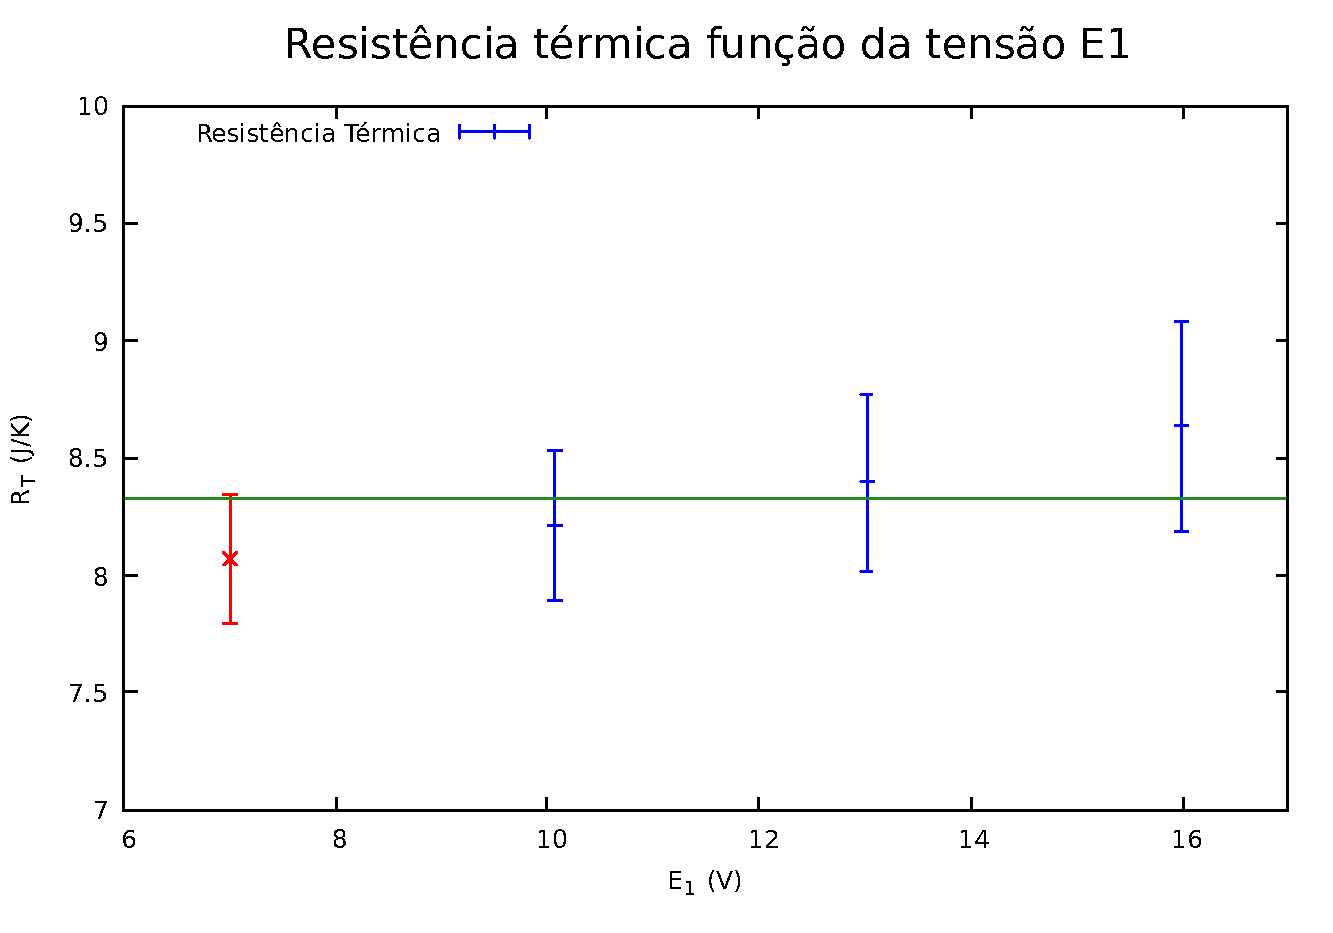
\includegraphics[width=240pt]{PreferidoDoRodrigo.pdf}
\par\noindent {\scriptsize ({\bf Gráfico 1}: Valores da resistência térmica para diferentes tensões $E_1$ e ajuste da equação \eqref{a}. O ponto mais à esquerda tem coordenadas $(7.00V,8.1J\K)$)}
\end{center}

\par Tendo-se obtido o seguinte resultado:

\begin{center}
\begin{tabular}{ x{2cm} x{2cm} }
\hline \hline
$a$ $(J/K)$ & 8.3$\pm$0.1 \tabularnewline
\hline \hline
\end{tabular}
\end{center}

\subsection*{Conversor termoelétrico como bomba de calor}

\par Efetuaram-se as alterações necessárias a obter a montagem representada na figura 2. De seguida, ajustou-se $E_1$ e $E_2$ por forma a colocar $I_2=0.5A$ e fazer com que a temperatura $T_a$ estabilizasse próximo dos $20^\circ C$. Atingido o equilíbrio, registaram-se as grandezas envolvidas, e repetiu-se o processo para $I=0.3A$. Obteve-se os seguintes resultados:

{\small
\begin{center}
\begin{tabular}{ x{1.5cm} x{2.2cm} x{2.2cm} }
$I_2$ $(mA)$ & 503.5$\pm$0.2 & 298.6$\pm$0.2 \tabularnewline
\hline \hline
$T_a$ $(^\circ C)$ & 18.606$\pm$0.004 & 16.9325$\pm$0.0005 \tabularnewline
$T_b$ $(^\circ C)$ & 28.03$\pm$0.03 & 24.418$\pm$0.002 \tabularnewline
$T_c$ $(^\circ C)$ & 23.48$\pm$0.02 & 22.87$\pm$0.03 \tabularnewline
$T_d$ $(^\circ C)$ & 22.589$\pm$0.006 & 22.651$\pm$0.007 \tabularnewline
$E_1$ $(V)$ & 6.160$\pm$0.001 & 3.451$\pm$0.001 \tabularnewline
$E_2$ $(A)$ & 7.660$\pm$0.001 & 4.609$\pm$0.001 \tabularnewline
$I_1$ $(A)$ & 0.307$\pm$0.001 & 0.172$\pm$0.001 \tabularnewline
$\dot{m}$ $(g/s)$ & 0.63$\pm$0.02 & 0.74$\pm$0.02 \tabularnewline
$P_1$ $(W)$ & 1.891$\pm$0.007 & 0.594$\pm$0.004 \tabularnewline
$P_1$ $(W)$ & 1.211$\pm$0.001 & 0.4440$\pm$0.0006 \tabularnewline
$P_3$ $(W)$ & 2.325$\pm$0.006 & 0.986$\pm$0.007 \tabularnewline
\end{tabular}
\par\noindent {\scriptsize ({\bf Tabela 6}: Parâmetros necessários ao cálculo da eficiência da bomba de calor)}
\end{center}
}

\par A partir destes valores, utilizaram-se as expressões \eqref{e} e \eqref{ec} para calcular a eficiência da bomba de calor e a eficiência ideal:

{\footnotesize
\begin{center}
\begin{tabular}{x{1.5cm} x{1.5cm} x{1.5cm} x{1.8cm}}
$I_2(mA)$ & $\varepsilon$ & $\varepsilon_c$ & $P_{perdas}$ $(W)$ \tabularnewline
\hline \hline
503.5 & 1.92$\pm$0.01 & 31.96$\pm$0.01 & 0.78$\pm$0.07\tabularnewline
298.6 & 2.22$\pm$0.02 & 39.75$\pm$0.01 & 0.05$\pm$0.07\tabularnewline
\end{tabular}
\par\noindent {\scriptsize ({\bf Tabela 7:} Valores das eficiências da bomba de calor e ideal e valor da potência de perdas)}
\end{center}
}


\section{Discussão dos Resultados}

\par Em primeiro lugar procedeu-se à verificação das temperaturas medidas para os diversos sensores a serem utilizados posteriormente ao longo da experiência. Uma vez que estes se encontravam em equilíbrio térmico, esperava-se que as temperaturas que indicavam fossem idênticas. Contudo, tal não se verificou - por conseguinte, procedeu-se à determinação da média dos valores obtidos e calculou-se o desvio em relação a esse valor para as temperaturas medidas por cada um dos sensores, tendo o valor obtido para cada um dos sensores sido adicionado ao valor medido por esse mesmo sensor no decurso da experiência por forma a garantir a fiabilidade dos resultados obtidos.

\par Relativamente à utilização do conversor termoeléctrico enquanto máquina térmica, procedeu-se primeiramente à determinação da resistência de carga óptima, para a qual se obteve um valor $R_{20}=(11.1\pm1.2)\ohm$. Uma vez que o valor máximo de resistência que podia ser atingido era $10\ohm$, o resto da experiência foi realizado tendo tal em conta. Procedeu-se então à determinação do valor do rendimento da máquina térmica para diferentes valores de tensão aplicada na célula de Peltier.

\par A primeira constatação obtida mediante a análise dos resultados obtidos consiste no facto de se ter verificado que um aumento de tensão implicaria um aumento da diferença de temperaturas entre a fonte quente e a fonte fria. Além disto, modelando o funcionamento do conversor termoeléctrico como sendo ideal, constata-se que o rendimento de Carnot aumenta consequentemente em função do aumento da tensão. Todavia, visto este sistema possuir um funcionamento real e, por conseguinte, serem-lhe inerentes perdas energéticas que deveremos considerar, foi efectuada a análise do rendimento $\eta_1$ considerando como potência fornecida $P_1$, isto é, a potência da fonte quente, e como potência útil $P_2$, isto é, a potência fornecida ao circuito pela célula de Peltier. O valor deste rendimento foi inferior ao de qualquer outro considerado ao longo do trabalho, indiciando a validade da análise efectuada, tendo sido ainda bastante inferior ao de Carnot, sendo que contudo o seu quociente diminui com o progressivo aumento da temperatura (para $U=7.00V$ e U=$15.99V$, o valor $\frac{\eta_C}{\eta_1}$ é de 14.5 e 12.9 respectivamente). Todavia, considerou-se ainda o caso de um rendimento para o qual seriam desprezadas perdas energéticas para o exterior, o que corresponderia a isolar o sistema (exequível, embora tais não fossem as condições proporcionadas no laboratório ao longo do decorrer da experiência). O rendimento $\eta_2$ resultante verifica ser simultaneamente superior a $\eta_1$ e inferior a $\eta_C$ para quaisquer valores de tensão, como seria de esperar.

\par É de notar que ao realizar a experiência o fluxo de água que actuava enquanto fonte fria se manteve constante para um valor todavia baixo. Tal resultou de material residual biológico que revestia o interior do tubo e que levava a uma diminuição do caudal, por um lado, e potenciava a formação de bolhas de ar por outro. Para evitar isto foi necessário ir continuamente modificando a posição do tubo, e manipular uma vez a própria célula, induzindo erros difíceis de controlar, visto as variações do caudal modificarem o contexto de execução da experiência. Para minimizar estes erros, mediu-se o fluxo durante um intervalo de tempo para o qual se mediram simultaneamente as temperaturas no início e no fim, permitindo fazer a média e ter em conta quaisquer flutuaçõesinerentes, reduzindo por conseguinte o erro associado. De facto, este procedimento foi efectuado para todas as medições de temperatura efectuadas ao longo da experiência.

\par Subsequentemente, procedeu-se à determinação de um novo rendimento denominado $\eta_3$ e que consistia em ignorar, além das perdas de energia para o exterior, as perdas de energia por condução. Tal conseguiu-se anulando-se no circuito a componente correspondente à célula de Peltier, calculando por conseguinte a resistência térmica inerente ao circuito e posteriormente a potência por condução. Assim, para os valores de tensão $7.00V$ e $15.99V$ obtiveram-se, respectivamente, os valores para a resistência térmica de $R_T=(8.1\pm0.3)K/W$ e $R_T=8.6\pm0.5K/W$. Embora esta teoricamente seja constante, notamos um desvio experimental. Todavia, caso consideremos um ajuste do tipo $R_T=a$ mediante o método dos mínimos quadrados, obtém-se um valor $a=(8.3\pm0.1)K/W$ e facilmente se verifica que ambos os valores se encontram englobados dentro do intervalo de incerteza experimental. De facto, após efectuar uma interpolação linear para os restantes valores, este valor encontra-se dentro da margem de erro de todos os valores experimentais. Efectuando o procedimento descrito obtiveram-se os novos valores deste rendimento, tendo estes sido superiores aos anteriores mas inferiores ao de Carnot, corroborando a análise efectuada.

\par Por fim, utilizou-se a máquina analisada desta vez enquanto bomba de calor por oposição à máquina térmica até agora estudada. De facto, para esta montagem, foi possível determinar o valor do COP para duas intensidades distintas de corrente através das diferenças de temperatura que lhes estavam associadas, tento o cuidado de no caso ideal considerar a temperatura em Kelvin visto não se tratar da sua diferença. Foi deste modo possível constatar que o valor do COP ideal era, tal como seria de esperar, demarcadamente superior em relação ao valor real, e que ambos aumentavam com a diminuição da diferença das temperaturas. De facto, verificou-se ainda que um aumento da intensidade de corrente leva a uma diminuição do valor do COP, o que é facilmente compreensível: um aumento da intensidade de corrente leva a uma aumento da tensão, o que por sua vez leva a um aumento da diferença de temperaturas, o que pelo previamente enunciado leva a uma diminuição do COP. Notamos no entanto uma menor disparidade, ainda que não sobremodo acentuada, entre os valores do COP ideais e teóricos e os valores dos rendimentos de Carnot e os experimentais previamente obtidos, sendo os ideiais sempre superiores aos experimentais. Tal é lógico, porquanto no caso real existem sempre perdas de energia, nomeadamente por condução para o exterior. De facto, foram calculadas as perdas energéticas e verficou-se que estas diminuiam acentuadamente para uma menor intensidade de corrente. De facto, as perdas por condução para o ar, por exemplo, são menores quando existe um menor gradiente de temperaturas, acentuadas pela aproximação entre as temperaturas medidas e a temperatura ambiente para o caso particular de $I=0.3A$ estudado.

\section{Conclusões}

\par Nesta experiência foi possível determinar o valor da resistência de carga óptima do circuito considerado, tendo-se obtido $R_{20}=(11.1\pm1.2)\ohm$. Obtiveram-se ainda valores para o rendimento do sistema em estudo enquanto máquina térmica para diferentes valores de tensão, tendo-se constatado que a um aumento de tensão correspondia um aumento do rendimento. Estes rendimentos foram quer ideiais quer reais, tendo em conta as várias possíveis formas de perdas e ganhos de energia pelo sistema, desde efeitos de condução ao de Peltier. Para este fim determinou-se um valor para a resistência térmica do sistema anulando o circuito pertinente à célula de Peltier, tendo este sido $R_T=(8.3\pm0.1)K/W$. Por fim, estudou-se o conversor termoeléctrico enquanto bomba de calor, tendo-se concluido que a menores intensidades de corrente correspondiam maiores valores do COP, porquanto a tal estão associados menores valores da diferença de temperaturas consideradas.

\par É de notar que a esta experiência se encontram associados diversos erros, alguns dos quais quase inevitáveis: erros de sensores, resistências internas desprezadas dos fios e diversos componentes eléctricos, um caudal inconstante e cuja inconstância é exacerbada por material biológico preenchendo o interior dos tubos de circulação da água. Para reduzir estes problemas foram tomadas várias medidas: medir a temperatura que os sensores assinalavam antes de efectuar a experiência e introduzir um factor correctivo, medir o caudal novamente para cada parte da experiência, e calcular a temperatura como a média dos valores registados no início e no fim da medição do caudal. Todavia, e embora isto tenha diminuido significativamente os erros verificados, esta experiência revela-se de difícil execução no tocante a obtenção rigorosa de resultados, sendo que poderia ser melhorada através da melhoria do equipamento apresentado e, evidentemente, de um maior intervalo de tempo ao longo do qual efectuar as medições por forma a obter valores mais estáveis no equilíbrio - particularmente porque é precisamente na análise de situações de equilíbrio que reside o âmago de toda esta experiência.


\begin{thebibliography}{9}

\bibitem{guia} Guia de objetivos do trabalho, Professor João Figueirinhas
\bibitem{apontamentos} Apontamentos das aulas teóricas
\bibitem{site} Wikipedia, the free encyclopedia - Thermoelectric effect. [Online] Available from: \url{http://en.wikipedia.org/wiki/thermoelectric\_effect}
\end{thebibliography}



\vfill

\pagebreak

%\section{Anexos}
%\subsection*{\normalsize Material}
%\begin{itemize}
%\item Cenas
%\end{itemize}
%
%\subsection*{\normalsize Tabelas Completas de Resultados}
%\par Cenas

\end{multicols}

\end{document}

% FOTOGRAFIA
%\begin{center}
%\includegraphics[width=240pt]{NOME SEM EXTENSAO}
%\par\noindent {\scriptsize (Figura X: Descrição)}
%\end{center}

%NOVA SUBSECÇÃO
%\subsection*{\normalsize BLA BLA}

%TABELA
%\begin{center}
%\begin{tabular}{ x{1.5cm} ... }
%i & ... \tabularnewline
%\hline \hline
%1 & 4.15  & 0.15  & 2033 & -  \tabularnewline
%\end{tabular}
%\par\noindent {\scriptsize (Tabela X: Descrição)}
%\end{center}